\chapter{表面重建} \label{chap3}
\section{引言}
为了计算表面张力,我们需要一种能够从点云中获取表面和表面法向的方法。本文使用的方法是
使用粒子水平集方法[**]获得一个粗糙的一阶连续隐式曲面,并使用MarchingCube[**]算法重构表面网格。然而该网格
的质量只能做到一阶连续,计算得到的法向在面片之间并不连续,难以应用在表面张力所需的法向计算。本文在该网格
上进行泊松圆盘采样,然后结合已经存在的IPIA算法,提出一种新的快速重建算法以此获得一个二阶光滑
的隐式曲面,然后基于该隐式曲面来计算表面点云的法向。
\section{粒子水平集方法}
记$\mathcal{V}$为点云集合,$v\in \mathcal{V}$为粒子,记$d(x,v)\in \mathbb{R}$为空间上$x$的点到粒子$v$的距离,
则$\mathcal{S}(v) = \{x\in \mathbb{R}^3: d(x,v) = r\}$为半径为$r$,圆心在$v$的球,如图\ref{fig:particle levelset}左所示,蓝色圆圈为二位情况的$\mathcal{S}(v)$。
\begin{figure}[htbp]
    \centering
    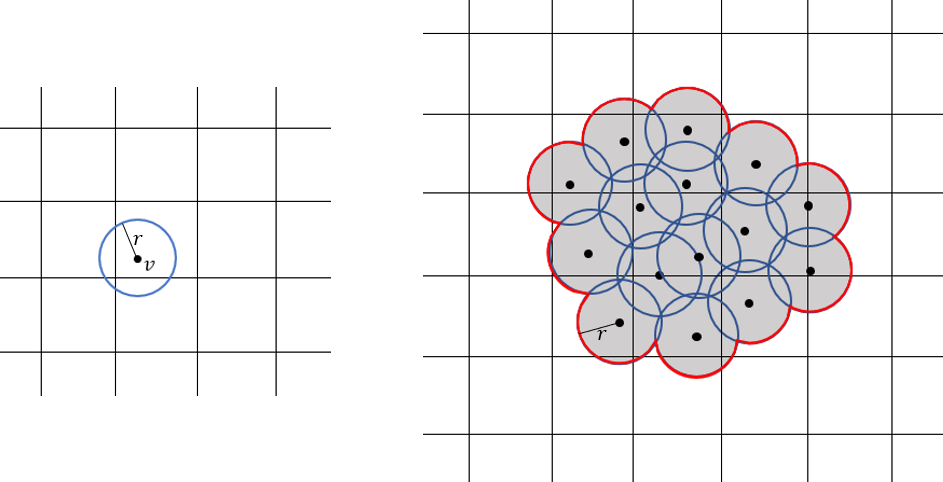
\includegraphics[scale=1.0]{./images/image3.png}
    \caption{二维情况$\mathcal{S}(v)$(左)与$\mathcal{S}(\mathcal{V})$(右)}
    \label{fig:particle levelset}
\end{figure}

记$d(x,\mathcal{V}):= \min \{ d(x,v): v\in \mathcal{V}\}$,则$\mathcal{S}(\mathcal{V}) = \{x\in \mathbb{R}^3: d(x,\mathcal{V}) = r\}$为点云的球外延边界。

如图\ref{fig:particle levelset}右所示,红色的外延边界为所求$\mathcal{S}(\mathcal{V})$。该红色边界初步确定了该点云的边界,灰色部分界定了物体内部。下一步我们将从利用红色边界和背景网格提取出
一个粗糙的网格。

\section{水平集网格提取}
Marching cube通常用于三维标量场的水平集的可视化,本文使用Marching cube算法来获取水平集的三角网格,在本文中我们的水平集为
$\mathcal{S}(\mathcal{V}) = \{x\in \mathbb{R}^3: d(x,\mathcal{V}) = r\}$。


\begin{figure}[htbp]
    \centering
    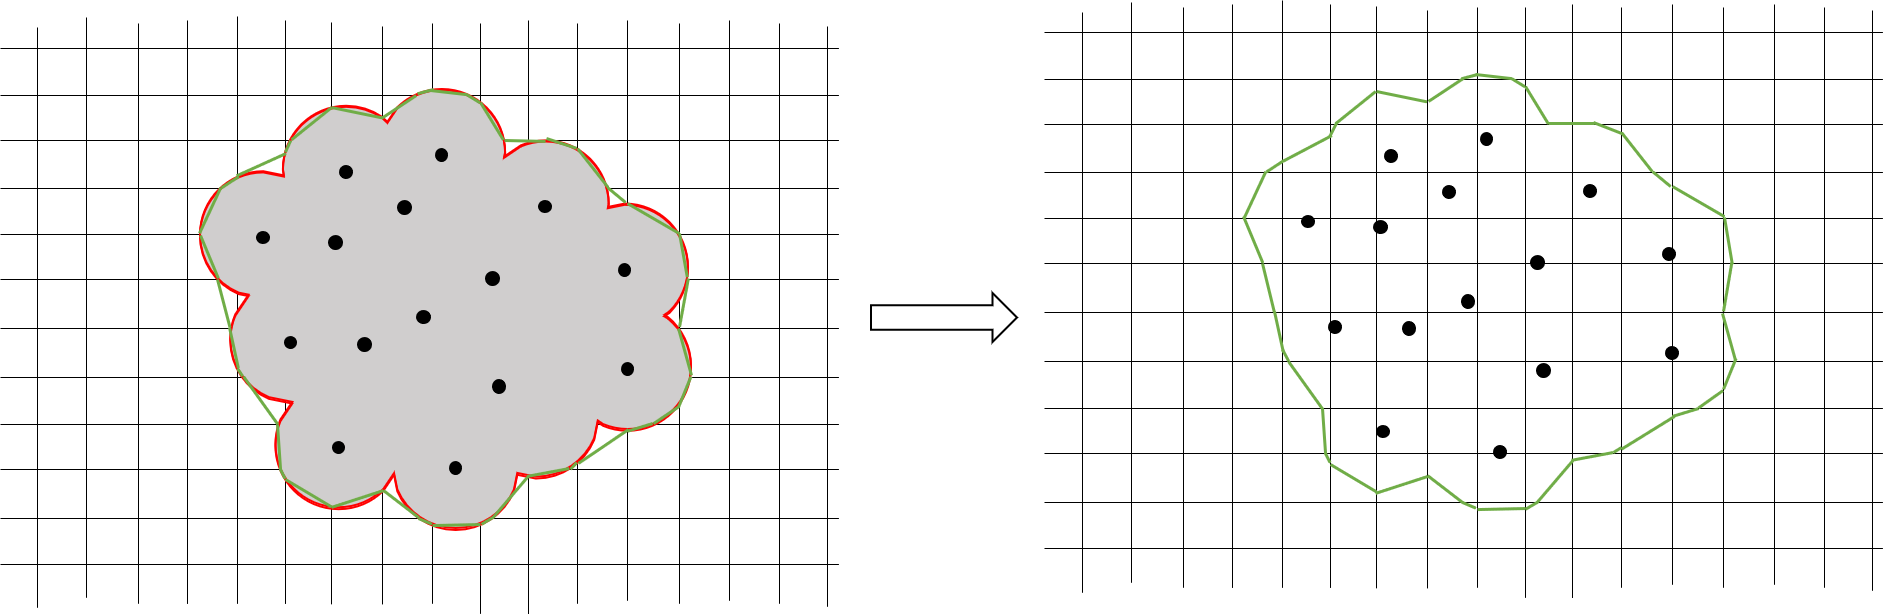
\includegraphics[scale=0.3]{./images/image7.png}
    \caption{二维点云轮廓提取图示}
    \label{fig:2D marching cube}
\end{figure}
\begin{figure}[htbp]
    \centering
    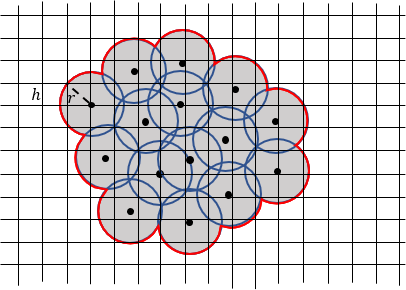
\includegraphics[scale=1.0]{./images/image5.png}
    \caption{二维情况的$r$与$h$的关系}
    \label{fig:grid and sphere}
\end{figure}

本小节我们的目标只是提取出一个大致的点云的表面轮廓,如图\ref{fig:2D marching cube}所示。我们首先将空间离散化成一个个均匀的立方体,并对每一个正方体格点放置一个标志符,默认为0,此处记立方体宽度为$h$,为了保证球能够覆盖到一个足够大的
面积,此处我们选择$r = \sqrt{3}h$,二维情况为$r = \sqrt{2}h$,具体如图\ref{fig:grid and sphere}所示。本文为了节省内存,
具体实现使用了八叉树数据结构。之后对每一个粒子操作,将粒子周围的格点做标记,如果格点距离该粒子半径不超过
$r$,则将格点标记为1,如此下来,所有的正方体格点都被标记为两种状态。之后我们对正方体按格点状态进行分类,由于每个格点有
两种状态,每个正方体有8个格点,如此一来便有$2^8 = 256$种状态,在合并旋转和对称的情况后,可以简化成15种,可以分类成如图\ref{fig:marching cube table}所示。
\begin{figure}[htbp]
    \centering
    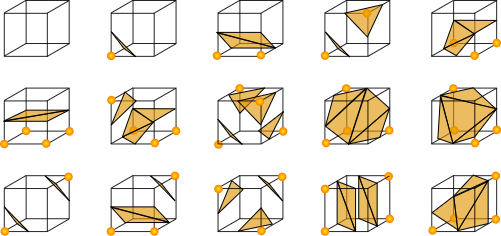
\includegraphics[scale=0.6]{./images/image6.png}
    \caption{Marching cube列表}
    \label{fig:marching cube table}
\end{figure}
之后我们再将网格顶点位置调整到合适的位置,并建立三角网格数据结构。具体算法见\ref{alg:marching cube}。
\begin{algorithm}
    \caption{Marching cube}
    \label{alg:marching cube}
    \begin{algorithmic}[1]
    \Require 点云集合$\mathcal{V}$,立方体宽度$h$
    \Ensure 三角网格位置集合$V$,面片集合$F$
    \State 准备空间网格数据结构(八叉树),并记$\mathcal{G}$为格点集合,$\mathcal{E}$为立方体的边集合,$\mathcal{C}$为立方体集合
    \State $state(g)\in \{0,1\}$为格点$g\in \mathcal{G}$的状态,初始化为0
    \State $P(e)\in \mathbb{R}^3$为边$e\in \mathcal{E}$上的一个顶点
    \State $r = \sqrt{3}h$
    \For{$v\in \mathcal{V}$}
        \For{$g \in \{g\in \mathcal{G}: \Vert g - v\Vert < r\}$}
            \State $state(g)$标记为1    
        \EndFor
    \EndFor    
    \For{$e \in \{e\in \mathcal{E}: e\text{两端格点状态相异}\}$}
      \State  取$e$状态为$1$的顶点记为$g_1$,状态为$0$的记为$g_0$
      \State 申请栈空间$p_{stack}$
      \For{$v \in \{v\in \mathcal{V}: \Vert g_1 - v\Vert < r\}$}
        \State 计算$\mathcal{S}(v)$与$e$的交点并压入$p_{stack}$中
      \EndFor
      \State 在$p_{stack}$中选取离$g_0$最近的点,并赋值给$P(e)$,同时将$P(e)$压入$V$中
    \EndFor
    \For{$c \in \mathcal{C}$}
        \State 匹配$c$所对应的Marching cube 列表中的状态
        \State 构造相应的三角面表$f_s$,顶点选为对应$P(e)$在$V$中得索引
        \State 将$f_s$其压入$F$中
    \EndFor
    \end{algorithmic}
\end{algorithm}


\textsf{在这里补点三维图,说明网格质量不行,只能一阶连续,法向不连续}


从实验结果的图中可以发现,Marching cube算法确实提取出了一个点云的边界轮廓,但是轮廓只能做到一阶连续,法向明显不连续,同时其三角网格质量无法
无法保证,甚至可以明显看出在一些尖锐地方,网格质量极差,上述的问题给我们计算表面张力带来了很大的阻碍。

\section{LSIPIA}
为了解决法向不连续的问题以及网格质量差的问题,我们使用隐式曲面来逼近三角网格。

\subsection{收敛性证明}